\chapter{Method}

\begin{enumerate}   \item Description of Node Copying as a method
  \begin{enumerate}     \item Node structure expansion
    \begin{enumerate}       \item Back pointers
      \item Modifications \item Bounds on numbers of the above \item How it
      works \item Why it works     \end{enumerate}
    \item Surrounding structure (collection of version information)
    \begin{enumerate}       \item Considerations about effecient storage and
    retrieval of version info     \end{enumerate}
  \end{enumerate}
  \item Description of ``Rollback'' as a method \begin{enumerate}     \item
  Description of reordering and optimization of operations (see algorithm
  \ref{alg:opsort} on page \pageref{alg:opsort})
  \end{enumerate}
  \item Definitions of various application profiles (how the DS is used)
  \end{enumerate}

\section{The Node Copying method}
Node Copying is a method described in \cite{Driscoll198986} by which a data
structure may be made partially persistent through the systematic expansion of
the nodes of the data structure. An auxillary data structure maintaining entry
points into the data structure, such as which node is the head of a linked list,
is also introduced. These two modifications of the data structure enable queries
to be made with $O(1)$ factor running time overhead and $O(1)$ space
consumption, given that the original data structure has an upper bounded
in-degree. In the following, I will describe in detail the general procedure as
well as giving the concrete example of the linked list.

\subsection{Node structure expansion}
As part of the Node Copying method, the node structure is expanded by adding two
arrays; one for ``back pointers'' and one for ``modifications''.

\begin{description}
  \item[Back pointers] 

  point back from a node $x$ to every node $y_i$ which points to $x$. When the
  in-degree has an upper bound, it is possible to restrict the size of the back
  pointers array. Whenever a node $y_i$ changes one of its pointers, the node
  $x$ it previously pointed to has the corresponding back pointer cleared, and
  the node $z$ it now points to has its corresponding back pointer set to point
  to $y_i$.

  \item[Modifications] store updates made to any of the fields of the node,
  including non-pointer fields, made since the node was created -- that is, the
  original field values from the time of construction remain unchanged. A
  modification record consist of a version number a field identifier and a
  value.

  When a field is to be modified on a node whose modifications array is already
  full, a copy of the node is constructed using the latest version of each field
  (including the one which is to be changed), thus resulting in a new node with
  an empty modifications array. The back pointers are also copied from the
  original node, and if the field being updated is a pointer field, the
  corresponding back pointer is updated in the destination node. This procedure
  is why the overall method is called Node Copying. A constant maximum number of
  modifications records is chosen such that node copying will have an amortized
  cost of $O(1)$.
\end{description}

\subsubsection{Amortized cost of Node Copying}
\todo[inline]{Write up proof of amortized time cost of node copying}

\section{Rollback}
Rollback is an approach to persistence based on the techniques described in
\cite{Tsotras1995237}, namely the combination of the na\"ive ``copy'' and
``log'' methods.
\subsection{The na\"ive approaches}
The ``copy'' approach makes a full copy of every version of the data structure
and makes it available by direct indexing to achieve $O(1)$ access overhead
factor. Creating each copy becomes more expensive in time and space the more
elements are inserted. In the worst case, when only insertions and no deletions
or modifications are made, the cost of creating $n$ versions is
$O\left(\binom{n+1}{2}\right)$.

The ``log'' approach conserves space by recording for each change made to the
data structure just enough information necessary to undo or redo it, thus giving
a space overhead factor per operation of $O(1)$. A ``current'' version
$v_{current}$ of the data structure is maintained. Given $v_{current}$, the
version $v_x$ can be produced by undoing or redoing all the changes between
$v_{current}$ and $v_x$ depending on which is the oldest. As the number of
versions $n$ increases, accessing a specific version becomes potentially more
costly. In the worst case, the overhead factor is $O(n)$ when $v_{current}$ is
$v_0$ and $v_x$ is $v_n$, or opposite.

\subsection{The hybrid approach}
An obvious hybrid of the two na\"ive approaches is to keep the records of each
operation like in the ``log'' approach, and storing a full copy like in the
``copy'' approach only at certain intervals. To access version $v_x$, the
nearest version to $v_x$ of which there exists a full copy, $v_s$, is retrieved.
Then, using the log of the versions from $v_s$ to $v_x$, the data structure
corresponding to $v_x$ is produced and returned.

Naturally, a user parameter is necessary to control the intervals at which full
copies are made. Let this parameter be $d$ and the number of versions $n$. There
will then be $\left\lfloor \frac{n}{d} \right\rfloor$ full copies, and the
maximum number of undos or redos to reach a specific version is then
$O(k+\frac{d}{2})$, where $k$ is the time required to retrieve the full copy. It
is now easy to see that the greater $d$ is, the fewer full copies will be made,
and thus the space cost is reduced accordingly. Likewise, the distance to the
version in the middle between two full copies increases with $d$, inducing a
higher cost for producing that version.

\subsubsection{Adaptive copy interval increase}
It might be preferrable to be able to specify a space usage limit rather than a
fixed interval distance. When the space limit is near, $d$ is increased by a
factor $c$, and the existing full copies are discarded except from every $c$
copy, thus freeing up space for additional full copies.

\todo[inline]{Insert figure illustrating adaptive copy interval increase.}

\subsection{Operations batch optimization}
For certain underlying data structures, it may prove to be feasible to
pre-process the batch of operations between a full copy $v_s$ and the requested
version $v_x$ in order to reduce the actual work necessary to reach $v_x$.

Two different types of pre-processing can be made to reduce work: Eliminating
superfluous operations and reordering operations. It is worth noting that both
of these require knowledge of the underlying data structure, and thus requires
more work to implement.

\subsubsection{Eliminating operations}
The batch of operations between $v_s$ and $v_x$ may contain some operations
which will not need to be explicitly applied. The cases are:
\begin{enumerate}
  \item An \textsc{insert} operation followed by a \textsc{remove} operation at
  the same effective index -- both can be removed from the batch since they
  cancel each other out.
  \label{item:elop-insert-remove}

  \item An \textsc{insert} operation followed by a \textsc{modify} operation at
  the same effective index -- the former can have its associated data value
  changed to that of the latter, and the latter can be removed from the batch.
  \label{item:elop-insert-modify}

  \item A \textsc{modify} operation followed by a \textsc{remove} operation at
  the same effective index -- the former can be removed from the batch.
  \label{item:elop-modify-remove}
\end{enumerate}

Cases \ref{item:elop-insert-remove} and \ref{item:elop-insert-modify} may of
course be combined in the sequence of one \textsc{insert} operation, one or more
\textsc{modify} operations and finally a \textsc{remove} operataion.

Pseudo code for an algorithm handling those cases is found in Algorithm
\ref{alg:eliminate-ops}.
The general idea is to identify cases \ref{item:elop-insert-remove},
\ref{item:elop-insert-modify} and \ref{item:elop-modify-remove} and make the
necessary maintenance before removing the relevant operations.

\begin{description}
  \item [Case \ref{item:elop-insert-remove}:] The operations between the
  \textsc{insert} operation and the \textsc{remove} operation are iterated to
  adjust the index on those operations which operate on indices greater than the
  index of the inserted element in the corresponding version.
  
  \item [Case \ref{item:elop-insert-modify}:] The \textsc{insert} operation gets
  the data value from the \textsc{modify} operation prior to the removal of the
  latter, and no further maintenance is necessary.
  
  \item [Case \ref{item:elop-modify-remove}:] The \textsc{modify} operation can
  simply be removed since it will have no net effect.

\end{description}

The space cost of the algorithm is in the order of the batch size, i.e.
$O(\left|B\right|)$, since a mutable copy of the relevant operations is made.
In the worst case, when all $n$ operations are \textsc{insert} or
\textsc{modify} operations, the time cost is $O\left(\binom{n+1}{2}\right)$,
since with every \textsc{insert} operation, all the proceeding operations are
examined when a matching \textsc{remove} operation is not found.

\begin{algorithm}[!ht]
  \caption{An algorithm for eliminating superfluous operations}
  \label{alg:eliminate-ops}
  \begin{algorithmic}[5]
    \Procedure{EliminateSuperfluousOps}{Batch $B$}
      \For {each operation $o_i \in B$, from last to first}
        \If {\textsc{type}($o_i$) $\in \left\{\textsc{insert},\textsc{modify}\right\}$}
        \State $c\gets\textsc{index}(o_i)$
          \For {each operation $o_j \in \left\{B|j>i\right\}$}
            \Switch {$\textsc{type}(o_j)$}
              \Case{\textsc{insert}}
                \If {$\textsc{index}(o_j) \le c$}
                  \State $c \gets c+1$
                \EndIf
              \EndCase
              \Case{\textsc{modify}}
                \If {$\textsc{index}(o_j) = c$}
                  \State $\textsc{data}(o_i) \gets \textsc{data}(o_j)$
                  \State remove $o_j$ from $B$
                \EndIf
              \EndCase
              \Case{\textsc{remove}}
                \If {$\textsc{index}(o_j) < c$}
                  \State $c \gets c-1$
                \ElsIf {$\textsc{index}(o_j) = c$}
                  \State $c \gets \textsc{index}(o_i)$
                  \Switch {$\textsc{type}(o_i)$}
                    \Case {\textsc{insert}}
                      \For {each operation $o_k \in \left\{B|i<k<j\right\}$}
                        \If {$\textsc{index}(o_k) > c$}
                          \State $\textsc{index}(o_k) \gets \textsc{index}(o_k) - 1$
                        \Else
                          \Switch {\textsc{type}($o_k$)}
                            \Case {\textsc{insert}}
                              \If {$\textsc{index}(o_k) \le c$}
                                \State $c \gets c+1$
                              \EndIf
                            \EndCase
                            \Case {\textsc{remove}}
                              \If {$\textsc{index}(o_k) \le c$}
                                \State $c \gets c-1$
                              \EndIf
                            \EndCase
                          \EndSwitch
                        \EndIf
                      \EndFor
                      \State remove $o_j$ from $B$
                      \State remove $o_i$ from $B$
                    \EndCase
                    \Case {\textsc{modify}}
                      \State remove $o_i$ from $B$
                    \EndCase
                  \EndSwitch
                \EndIf
              \EndCase
            \EndSwitch
          \EndFor
        \EndIf
      \EndFor
    \EndProcedure
  \end{algorithmic}
\end{algorithm}
 
\subsubsection{Reordering operations}

Applying each operation in the batch separately is potentially a time-expensive
approach. Consider the case when each operation inserts an element at the end of
a linked list; the bulk cost for $n$ insertions on a list of length $l$ would be

$$O\left(\dbinom{l+n+1}{2}\right)$$

since every insertion would require following 1 more pointer than the previous.
It would indeed be more efficient to make the insertions in one go, which would
cost $O(l+n)$ -- $l$ for reaching the end of the list, $n$ for all the
insertions. But this is only possible if the the operations are ordered by
non-decreasing index of application. If they are not, they can be reordered.

Reordering the batch of operations by index of application requires some
maintenance. Consider the case when an \textsc{insert} operation $o_i$, which
has a small index of application, is moved to an earlier position in the batch
than it had originally. Any operations which used to preceed $o_i$, and which
after the move will instead proceed it, should take into account the additional
element being inserted; if their index of application is greater than that of
$o_i$, it should be incremented by 1. If $o_i$ is a \textsc{remove} operation,
the index of operation should instead be decreased by 1 on those operations.

Pseudocode for an algorithm implementing the above approach is found in
Algorithm \ref{alg:opsort}. The space cost is linear in the number of operations
being reordered. Consider the worst case, when the operations are ordered with
strictly decreasing indices of application; the time cost is then
$O\left(\binom{n+1}{2}\right)$, since the entire remaining sequence would have
to be searched for the minimum index of application prior to the removal of that
element.

An example of the reordering of 10 operations by the algorithm is found in
figure \ref{fig:reorder-example}.

\begin{figure}[!htp]
  \includegraphics[width=.9\textwidth]{figures/reorder_example.pdf}

  \caption{\small Example of the reorder algorithm applied to a sequence of 10
  operations. In each iteration, the minimum operation in $S$ is colored cyan.
  When an \textsc{insert} operation is removed from $S$, the operations to the
  left are colored green to indicate the incrementation of their label.
  Similarly, when a \textsc{remove} operation is removed from $S$, the
  operations to the left are colored red to indicate the decrementation of their
  label.}

  \label{fig:reorder-example}
\end{figure}

If the operations are already ordered by non-decreasing index of application,
the algorithm only adds to the time cost, and so it may be worth checking that
the sequence requires reordering prior to running the algorithm. That can be
achieved in $O(n)$ time by testing whether each operation works on an index
equal to or greater than the previous one.

\paragraph {Proof of reorder algorithm}
\begin{definition}
\label{def:reorder-iter}

Let $S_0$ be the original sequence and let $O_0$ be an empty sequence at the
beginning of the first iteration. By definition, the sequence $O_0$, $S_0$
corresponds to $S_0$. At the beginning of iteration $i$, let $l_{min_i}$ be the
minimum index of any operation in $S_i$, and let $o_{min_i}$ be the left-most
operation in $S_i$ with such index. Let $L_i$ be the operations to the left of
$o_{min_i}$ in $S_i$, and $R_i$ those to the right.

\end{definition}

\begin{lemma}
\label{lem:reorder-inequality}

By definition \ref{def:reorder-iter}, at the beginning of iteration $i$, all
operations in $L_i$ have greater indices than $o_{min_i}$, and no operations in
$R_i$ have lower indices than $o_{min_i}$.

\end{lemma}

\begin{theorem}
\label{theorem:reorder-swap}

Let operation $o_b$ directly follow $o_a$ in a sequence. If $o_b$ works on a
higher index than $o_b$, swapping $o_a$ and $o_b$ in the sequence will have no
consequence for the outcome. If, on the other hand, $o_b$ works on a lower index
than $o_a$, letting $o_b$ be applied before $o_a$ will potentially shift the
elements in the list on which the operations work, and $o_a$ will subsequently
work on the wrong element unless compensation is made.

Specifically, if $o_b$ is an \textsc{insert} operation, $o_a$ should be
compensated by incrementing by 1 the index on which it works, and by
decrementing it by 1 if $o_b$ is a \textsc{remove} operation. If $o_b$ is a
\textsc{modify} operation, it does not shift the elements in the list, and as
such that case can be disregarded.

As a result, applying $o_a$, then $o_b$ corresponds to (yields the same result
as) applying $o_b$, then the compensated $o_a$.

Similarly, once $o_b$ has been swapped with $o_a$ and $o_a$ compensated, $o_b$
may again be swapped with any operation to its left.

\end{theorem}

\begin{theorem}

Let
\begin{equation*}
t_i = 
\begin{cases}
    1, & \text{if $\textsc{type}(o_{min_i}) = \textsc{insert}$}.\\
    0, & \text{if $\textsc{type}(o_{min_i}) = \textsc{modify}$}.\\
    -1, & \text{if $\textsc{type}(o_{min_i}) = \textsc{remove}$}.
\end{cases}
\end{equation*}

and $Lr_i$ be $L_i$ with the index of each operation adjusted by $t_i$.

Then by lemma \ref{lem:reorder-inequality} and theorem
\ref{theorem:reorder-swap}, applying the $L_i$, then $o_{min_i}$ corresponds to
applying $o_{min_i}$, then $Lr_i$, since all operations in $L_i$ would have to
be compensated if $o_{min_i}$ is swapped with each operation, seeing that they
have greater indices than $o_{min_i}$ does.

Since the result of applying $o_{min_i}$, then $Lr_i$ corresponds to applying
$L_i$, then $o_{min_i}$, no operations in $R_i$ need adjustment.

If before the next iteration $O_{i+1}$ is set to $O_i$ followed by $o_{min_i}$
and $S_{i+1}$ is set to $S_i$ with $o_{min_i}$ removed, it follows that applying
$O_{i+1}$, then $S_{i+1}$ corresponds to applying $O_i$, then $S_i$.

\end{theorem}

\begin{proof}

In each iteration after $i=0$, the size of $S_i$ is smaller by 1 than $S_{i-1}$,
until the last iteration in which $S_i$ is empty and the algorithm terminates by
returning $O_i$.

Since in the end of each operation, the operation with the minimum index is
transferred from $S_i$ to the back of $O_{i+1}$, the operations in $O_i$ are
ordered by non-decreasing index.

In the last iteration, $O_i$ will contain operations corresponding to those in
$S_0$, but in a non-decreasing order and compensated for their new order in the
sequence such that the result of applying it will be the same as $S_0$. \qed

\end{proof}

\begin{algorithm}[!ht]
  \caption{Algorithm for sorting a set of operations}
  \label{alg:opsort}
  \begin{algorithmic}[5]
    \Function {SortOperations}{set of operations $B$}
      \State result $\gets$ empty set
      \While {$B$ not empty}
        \State // Find left-most operation with minimum index of application
        \State $o_{min} \gets$ op. with minimum index of application
        \State $index_{min} \gets$ index in $B$ of $o_{min}$
        \State \textsc{remove} $o_{min}$ from $B$
        \State \textsc{append} $o_{min}$ to result
        \Statex
        \State // Compensate op.s which will now proceed rather than
        preceed $o_{min}$
        \For {each op. $o_i\in \left\{B | 0\le i<index_{min}\right\}$ }
          \If {$o_{min}$ is an \textsc{insert} op.}
                \State \textsc{index}($o_i$) $\gets$ \textsc{index}($o_i$) + 1
          \ElsIf {$o_{min}$ is a \textsc{remove} op.}
                \State \textsc{index}($o_i$) $\gets$ \textsc{index}($o_i$) - 1
          \EndIf
        \EndFor
       \EndWhile
      \Statex
      \State \Return result
    \EndFunction
  \end{algorithmic}
\end{algorithm}
